
\documentclass[
	% -- opções da classe memoir --
	12pt,				% tamanho da fonte
	openright,			% capítulos começam em pág ímpar (insere página vazia caso preciso)
	oneside,			% para impressão em verso e anverso. Oposto a oneside
	a4paper,			% tamanho do papel. 
	% -- opções da classe abntex2 --
	%chapter=TITLE,		% títulos de capítulos convertidos em letras maiúsculas
	%section=TITLE,		% títulos de seções convertidos em letras maiúsculas
	%subsection=TITLE,	% títulos de subseções convertidos em letras maiúsculas
	%subsubsection=TITLE,% títulos de subsubseções convertidos em letras maiúsculas
	% -- opções do pacote babel --
	english,			% idioma adicional para hifenização
	brazil				% o último idioma é o principal do documento
	]{abntex2}

% ---
% Pacotes básicos 
% ---
%\usepackage{uarial}				% Usa a fonte Latin Modern			lmodern
\usepackage[T1]{fontenc}		% Selecao de codigos de fonte.
\usepackage[utf8]{inputenc}		% Codificacao do documento (conversão automática dos acentos)
\usepackage{lastpage}			% Usado pela Ficha catalográfica
\usepackage{indentfirst}		% Indenta o primeiro parágrafo de cada seção.
\usepackage{color}				% Controle das cores
\usepackage{graphicx}			% Inclusão de gráficos
\usepackage{microtype} 			% para melhorias de justificação
\usepackage{float}
\usepackage{babel}

\usepackage{fancyvrb}
\usepackage{minted}
\newminted{python}{frame=lines,framerule=2pt}

\usepackage[font=small,labelfont=bf]{caption}


% pacotes adicionados
\usepackage{amsmath}
\usepackage{amssymb,amsfonts,amsthm}
\usepackage{setspace}
% ---

\usepackage{listings}
\usepackage{xcolor}
\usepackage{inconsolata}
\lstset{
    language=bash, %% Troque para PHP, C, Java, etc... bash é o padrão
    basicstyle=\ttfamily\small,
    numberstyle=\footnotesize,
    numbers=left,
    backgroundcolor=\color{gray!10},
    frame=single,
    tabsize=2,
    rulecolor=\color{black!30},
    title=\lstname,
    escapeinside={\%*}{*)},
    breaklines=true,
    breakatwhitespace=true,
    framextopmargin=2pt,
    framexbottommargin=2pt,
    inputencoding=utf8,
    extendedchars=true,
    literate={á}{{\'a}}1 {ã}{{\~a}}1 {é}{{\'e}}1,
}
		
% ---
% Pacotes adicionais, usados apenas no âmbito do Modelo Canônico do abnteX2
% ---
\usepackage{lipsum}				% para geração de dummy text
% ---
\usepackage{todonotes}
% ---
% Pacotes de citações
% ---
\usepackage[brazilian,hyperpageref]{backref}	 % Paginas com as citações na bibl
\usepackage[alf]{abntex2cite}	% Citações padrão ABNT


\renewcommand{\bf}[1]{\mathbf{#1}}
\renewcommand{\rm}[1]{\mathrm{#1}}


\usepackage{cite}
\renewcommand\citeleft{[}
\renewcommand\citeright{]}

% --- 
% CONFIGURAÇÕES DE PACOTES
% --- 
%\renewcommand{\imprimircapa}{
%\thispagestyle{empty}

\vfill
 \begin{center}
    
    {\large\bfseries INSTITUTO FEDERAL DE MATO GROSSO DO SUL} \\
    
    {\large\bfseries CAMPUS NAVIRAÍ}  \\ 

    \vspace*{1in}

    \vspace*{4cm}
    \noindent \\
    
    \large\bfseries{NOTAS DE AULA DE} \\
    \huge\bfseries{LINGUAGEM DE APRESENTAÇÃO E ESTRUTURAÇÃO DE CONTEÚDOS} \\ I
    
    \vspace*{4cm}
    
    \large{Prof. MSc. Luiz F. Picolo}
    
    \vfill
    \large\bfseries{NAVIRAÍ - MS} \\ 
    \vspace{0.2cm}
    \small Atualizado em \today
\end{center}

\normalsize


}


% \renewcommand{\imprimirfolhaderosto}{
% \include{folhaderosto}}


% ---
% Configurações do pacote backref
% Usado sem a opção hyperpageref de backref
\renewcommand{\backrefpagesname}{Citado na(s) página(s):~}
% Texto padrão antes do número das páginas
\renewcommand{\backref}{}
% Define os textos da citação
\renewcommand*{\backrefalt}[4]{
	\ifcase #1 %
		Nenhuma citação no texto.%
	\or
		Citado na página #2.%
	\else
		Citado #1 vezes nas páginas #2.%
	\fi}%
% ---
% \include{capa}

% ---
% Configurações de aparência do PDF final

% alterando o aspecto da cor azul
\definecolor{blue}{RGB}{41,5,195}

% informações do PDF
\makeatletter
\hypersetup{
     	%pagebackref=true,
		colorlinks=true,       		% false: boxed links; true: colored links
    	linkcolor=blue,          	% color of internal links
    	citecolor=black,        		% color of links to bibliography
    	filecolor=magenta,      		% color of file links
		urlcolor=blue,
		bookmarksdepth=4
}



\makeatother
% --- 

% --- 
% Espaçamentos entre linhas e parágrafos 
% --- 

% O tamanho do parágrafo é dado por:
\setlength{\parindent}{1.3cm}

% Controle do espaçamento entre um parágrafo e outro:
\setlength{\parskip}{0.2cm}  % tente também \onelineskip

% ---
% compila o indice
% ---
% \makeindex
% ---

% ----
% Início do documento
% ----
\begin{document}

% Seleciona o idioma do documento (conforme pacotes do babel)
%\selectlanguage{english}
\selectlanguage{brazil}

% Retira espaço extra obsoleto entre as frases.
\frenchspacing 

% ----------------------------------------------------------
% ELEMENTOS PRÉ-TEXTUAIS
% ----------------------------------------------------------
\pretextual

% ---
% Capa
% ---
\thispagestyle{empty}

\vfill
 \begin{center}
    
    {\large\bfseries INSTITUTO FEDERAL DE MATO GROSSO DO SUL} \\
    
    {\large\bfseries CAMPUS NAVIRAÍ}  \\ 

    \vspace*{1in}

    \vspace*{4cm}
    \noindent \\
    
    \large\bfseries{NOTAS DE AULA DE} \\
    \huge\bfseries{LINGUAGEM DE APRESENTAÇÃO E ESTRUTURAÇÃO DE CONTEÚDOS} \\ I
    
    \vspace*{4cm}
    
    \large{Prof. MSc. Luiz F. Picolo}
    
    \vfill
    \large\bfseries{NAVIRAÍ - MS} \\ 
    \vspace{0.2cm}
    \small Atualizado em \today
\end{center}

\normalsize



% ---

% ---
% Folha de rosto
% (o * indica que haverá a ficha bibliográfica)
% ---
% \imprimirfolhaderosto

% \include{ficha}
%\include{errata}
% \include{folhaaprova}
%\include{dedicatoria}
% \include{agradecimentos}
%\include{epigrafe}
% \include{resumos}
% ---
% inserir lista de ilustrações
% ---
% \pdfbookmark[0]{\listfigurename}{lof}
% \listoffigures*
% \cleardoublepage
%% ---

% ---
% inserir lista de tabelas
% ---
% \pdfbookmark[0]{\listtablename}{lot}
% \listoftables*
% \cleardoublepage
% ---
% \include{siglas}
% ---
% inserir o sumario
%% ---
% \pdfbookmark[0]{\contentsname}{toc}
%\tableofcontents*
%\cleardoublepage
%% ---



% ----------------------------------------------------------
% ELEMENTOS TEXTUAIS
% ----------------------------------------------------------
\textual

\chapter{Introdução}\label{cap:cap_01}

\begin{flushright}
	\textit{
		Professores podem abrir a porta, mas você \\ precisa passar por ela por você mesmo. 
	} \\
	
	\textbf{Provérbio Chinês}
\end{flushright}
\chapter{Client-Side e Server-Side}\label{cap:cap_02}

\begin{flushright}
	\textit{
		Viva como se fosse morrer amanhã. \\ Aprenda como se fosse viver para sempre.
	} \\
	\textbf{Mahatma Gandhi}
\end{flushright}

Client-Side (Lado do cliente) e Server-Side (lado do servidor) são dois termos importantes envolvidos no desenvolvimento de software e web. As duas categorias de desenvolvimento têm muitas diferenças, incluindo diferentes propósitos e linguagens de programação. Assim, como nosso objetivo é trabalhar com o desenvolvimento de software, é importante que possamos  entender o desenvolvimento tanto do lado do cliente quanto a do lado do servidor. Assim, nossa jornada se inicia entendendo um dos lados, o do servidor, a qual fará parte do nosso curso durante nossos próximo três semestre. 

\section{O que é desenvolvimento do lado do cliente?}

O desenvolvimento do lado do cliente é uma categoria de desenvolvimento que envolve programas executados em um cliente ou dispositivo do usuário. Os(as) desenvolvedores(as) do lado do cliente se concentram em criar a parte de um sistema com a qual o usuário pode interagir. Às vezes, o desenvolvimento do lado do cliente também é chamado, erroneamente, de desenvolvimento \textbf{front-end}, pois se concentra na parte ``frontal'' de um aplicativo que os usuários podem ver. Os(as) desenvolvedores(as) do lado do cliente concluem uma variedade de tarefas, incluindo:

\begin{itemize}[leftmargin=1.7cm]
	\setlength\itemsep{0em}
	\item Criação de layouts de sites
	\item Projetando interfaces de usuário
	\item Adicionando validação de formulário
	\item Adicionando elementos visuais como cores e fontes
\end{itemize}

Pessoas que desenvolvem para o lado do cliente se preocupam com a experiência do usuário e usam linguagens de programação específicas. Algumas linguagens comuns do lado do cliente incluem:

\begin{itemize}[leftmargin=1.7cm]
	\setlength\itemsep{0em}
	\item  O \textbf{HTML}, que significa\textit{ Hypertext Markup Language}, é uma linguagem de marcação padrão para desenvolvimento web. HTML constrói a estrutura de um site o renderiza em um navegador.
	
	\item O \textbf{CSS}, que significa \textbf{Cascading Style Sheets}, é uma linguagem de design que os(as) desenvolvedores(as) podem usar para adicionar elementos de design visual a um site codificado em HTML. Os desenvolvedores podem usar CSS para tornar seus sites visualmente atraentes nos dispositivos dos usuários.
	
	\item Já o \textbf{JavaScript} é uma linguagem de programação que os(as) desenvolvedores(as) podem usar para desenvolvimento web, aplicações web e outros propósitos. Os\textbf{} desenvolvedores\textbf{} podem usar \textbf{JavaScript} para tornar os sites dinâmicos e interativos. 
\end{itemize}

Contudo, nos últimos anos, JavaScript se tornou uma linguagem que também pode ser usado do lado do servidor dando ao desenvolvedor(a) maior alcance com o conhecimento adquirido. Contudo, mesmo sendo a mesma linguagem, o objetivo acaba diferindo, por isso, vamos entender melhor como usar o JavaScript do lado do servidor. 

\section{O que é desenvolvimento do lado do servidor?}

O desenvolvimento do lado do servidor é um categoria de desenvolvimento que envolve programas executados em um servidor. Os(as) desenvolvedores(as) do lado do servidor se concentram no desenvolvimento nos bastidores, e o desenvolvimento do lado do servidor também é conhecido, e nesse caso acertadamente, como desenvolvimento ``back-end''. Esse categoria de programação é importante porque os navegadores da Web, ou clientes, interagem com os servidores da Web para recuperar informações. 

\begin{figure}[H]
	\centering
	\caption{Client-Side e Server-Side}
	\frame{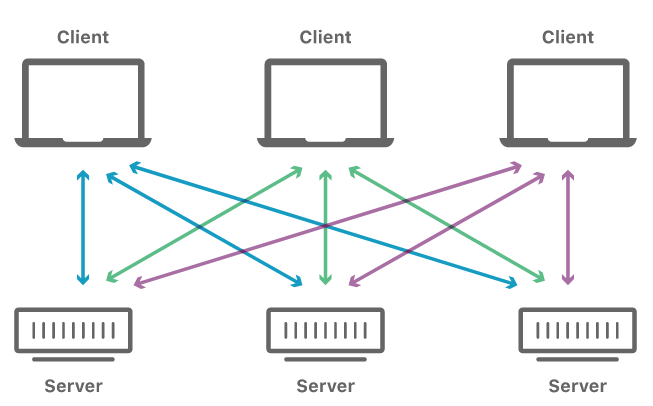
\includegraphics[scale=0.4]{imagens/csss.png}}
	\legend{\textbf{Fonte}: \url{https://bityli.com/jwImTW}}
\end{figure}

As tarefas comuns do lado do servidor incluem:

\begin{itemize}[leftmargin=1.7cm]
	\setlength\itemsep{0em}
	\item Codificando sites dinâmicos
	\item Desenvolvendo aplicações web
	\item Conectando sites a bancos de dados
\end{itemize}

Desenvolvedores(as) de software, administradores(as) de banco de dados e desenvolvedores(as) da Web normalmente usam o desenvolvimento do lado do servidor. Os desenvolvedores do lado do servidor podem usar muitas linguagens de programação diferentes, tais como \textbf{PHP}, \textbf{Java}, \textbf{SQL} e também \textbf{JavaScript} a qual será a linguagem base que usaremos no decorrer do curso.

\section{Lado do cliente vs. lado do servidor}

Lado do cliente e lado do servidor são termos que indicam como e onde o código é executado. Alguns desenvolvedores, chamados desenvolvedores \textbf{full-stack}, sabem como usar o desenvolvimento do lado do cliente e do lado do servidor, pois ambos são importantes para o funcionamento de sites e aplicativos. No entanto, existem algumas diferenças importantes entre o desenvolvimento do lado do cliente e do lado do servidor. Algumas das principais diferenças entre os dois tipos de desenvolvimento incluem:

\subsection{Onde o código é executado?}

Uma grande diferença entre o desenvolvimento do lado do cliente e do lado do servidor é onde o código é executado. No desenvolvimento do lado do cliente, o código é executado no dispositivo do cliente ou do usuário. No entanto, no desenvolvimento do lado do servidor, o código é executado por meio de um servidor. É por isso que o desenvolvimento do lado do cliente também é chamado de front-end e o desenvolvimento do lado do cliente também é back-end.

\subsection{Como é executado?}

A maneira como os códigos são executados é outra diferença entre o desenvolvimento do lado do cliente e do lado do servidor. No código do lado do cliente, o código são simplesmente executados em um dispositivo, muitas vezes em um navegador com pouco ou nenhum acesso à memória do computador. Já do lado do servidor, no entanto, são executados em um servidor web com total acesso à memória do computador.

\subsection{Quais as Finalidades?}

O desenvolvimento do lado do cliente e do lado do servidor também têm propósitos diferentes. O principal objetivo do desenvolvimento do lado do cliente é criar efeitos visuais de sites, incluindo layouts, interfaces de usuário, validação de formulários e outros elementos visuais. O desenvolvimento do lado do servidor, no entanto, concentra-se mais no conteúdo real de uma página da Web e conclui tarefas como interagir com bancos de dados e recuperar informações de um servidor da Web.

\section{Protocolo HTTP}

Um protocolo é um sistema de regras que define como os dados são trafegados dentro ou entre computadores. Comunicações entre dispositivos requer que estes concordem com o formato do dado que estiver sendo trafegado. O conjunto de regras que define esse formato é chamado protocolo.

Podemos representar um protocolo como um meio de comunicação comum a dois indivíduos que não são falantes do mesmo idioma. Assim, uma das maneiras para que a comunicação aconteça e que ambos falem um idioma comum, como, por exemplo, o inglês. Clientes e servidores se comunicam trocando mensagens individuais. As mensagens enviadas pelo cliente, geralmente um navegador da Web, são chamadas de solicitações (requests), ou também requisições, e as mensagens enviadas pelo servidor como resposta são chamadas de respostas (responses).

\begin{figure}[H]
	\centering
	\caption{Analogia Protocolo}
	\frame{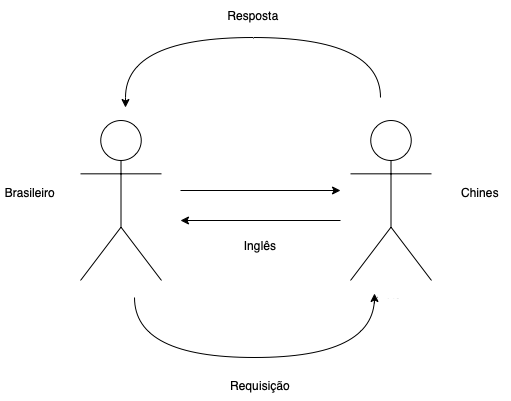
\includegraphics[scale=0.4]{imagens/protocolo.png}}
	\legend{Fonte: O autor}
	\label{fig:protocolo}
\end{figure}

Assim, o HTTP (\textit{Hypertext Transfer Protocol}) segue a mesma dinâmica. O HTTP é um protocolo que permite a obtenção de recursos, como documentos HTML. É a base de qualquer troca de dados na Web e um protocolo cliente-servidor, o que significa que as requisições são iniciadas pelo destinatário, geralmente um navegador da Web. Um documento completo é reconstruído a partir dos diferentes sub-documentos obtidos, como, por exemplo texto, descrição do layout, imagens, vídeos, scripts e muito mais.

\subsection{Métodos de requisição HTTP}

O protocolo HTTP define um conjunto de métodos de requisição responsáveis por indicar a ação a ser executada para um dado recurso. Embora esses métodos possam ser descritos como substantivos, eles também são comumente referenciados como \textit{HTTP Verb}s (Verbos HTTP). O HTTP implementa vários verbos, porém, os mais usados são:

\begin{itemize}[leftmargin=1.7cm]
	\setlength\itemsep{0em}
	\item \textbf{GET}: O método GET solicita a representação de um recurso específico. Requisições utilizando o método GET devem retornar apenas dados.
	\item \textbf{POST}: O método POST é utilizado para submeter uma entidade a um recurso específico, frequentemente causando uma mudança no estado do recurso ou efeitos colaterais no servidor.
	\item \textbf{PUT}: O método PUT substitui todas as atuais representações do recurso de destino pela carga de dados da requisição.
	\item \textbf{DELETE}: O método DELETE remove um recurso específico.
\end{itemize}

\section{Exercícios de fixação}

\begin{enumerate}[leftmargin=1.7cm]
	\setlength\itemsep{0em}
	\item Qual a diferença entre ``Client-Side (lado do cliente) e Server-Side (Lado do servidor)"?
	\item O que é um protocolo e, por que ele é usado na comunicação?
	\item Explique o que é um Verbo HTTP e como eles são utilizados na comunicação.
	\item O JavaScript é uma linguagem Client-Side ou Server-Side? Explique sua resposta.
\end{enumerate}
\chapter{Servidor Web com NodeJS}\label{cap:cap_03}

\begin{flushright}
	\textit{
		As raízes do estudo são amargas, \\ mas seus frutos são doces.
	} \\
	\textbf{Aristóteles}
\end{flushright}

Ao acessar e visualizar uma página em seu navegador, como, por exemplo \url{https://www.ifms.edu.br}, você está fazendo uma solicitação (request) a outro computador na rede (ou internet), que em resposta (response), fornece a você a página Web. O computador que está se comunicando por meio da sua solicitação executa uma aplicação que é o \textbf{servidor Web}. Um servidor Web recebe solicitações HTTP de um \textbf{cliente}, como seu navegador, e fornece uma resposta HTTP, como uma página HTML.

O \textbf{Node.js} permite que os desenvolvedores utilizem o JavaScript para escrever o código do lado do servidor (Server-Side), embora ele seja tradicionalmente usado no navegador para escrever o código do lado do cliente (Client-Side). Assim, vamos aprender como desenvolver servidores Web usando o módulo http que está incluído no Node.js que poderá retornar dados em JSON, arquivos CSV e páginas Web em HTML.

\section{Criando um servidor HTTP básico}

Para iniciarmos a configuração vamos criar um servidor que retorna um texto sem formatação ao usuário. Primeiro, precisamos configurar um ambiente de programação acessível para fazer nossos exercícios. Para tanto, vamos criar e acessar uma pasta chamada \textbf{primeiro-servidor}:

\begin{minted}[frame=single,framesep=10pt,breaklines,linenos,tabsize=2,autogobble]{javascript}
mkdir primeiro-servidor
cd primeiro-servidor
\end{minted}

Dentro do diretório vamos criar um arquivo com o nome de \textbf{index.js} e nele iniciaremos as primeiras linhas para a implementação do nosso servidor HTTP. Começaremos carregando o módulo \textbf{http}, padrão em todas as instalações do Node.js. Adicione a linha seguinte ao \textbf{index.js}:

\begin{minted}[frame=single,framesep=10pt,breaklines,linenos,tabsize=2,autogobble]{javascript}
const http = require("http");
\end{minted}

Nosso próximo passo definiremos duas constantes, o \textbf{host} e a \textbf{porta} em que nosso servidor se associará. O \textbf{host} nada mais é do que o ``endereço'' que faremos o acesso ao servidor e a \textbf{porta} pode ser qualquer número entre 1024 até 40.000. Contudo, por padrão, vamos usar a porta 8080.

\begin{minted}[frame=single,framesep=10pt,breaklines,linenos,tabsize=2,autogobble]{javascript}
const http = require("http");

const host = 'localhost';
const porta = 8080;
\end{minted} 

Como mencionado anteriormente, os servidores Web aceitam solicitações de navegadores e de outros clientes. Podemos interagir com um servidor Web ao digitar um nome de domínio. O valor \textbf{localhost} é um endereço privado especial que os computadores utilizam para se referir a eles mesmos. Normalmente, ele é equivalente ao endereço \textbf{IP interno 127.0.0.1} e está disponível apenas para o computador local, ou seja, não está disponível para nenhuma rede local da qual participamos ou para a Internet. Por fim, definimos a porta, que é o número que representa o ``local'' no computador onde o servidor está sendo executado. 

Ao vincularmos nosso \textbf{servidor} a este \textbf{host} e \textbf{porta}, conseguiremos acessar nosso servidor ao visitarmos http://localhost:8080 em um navegador local.

Vamos adicionar uma função especial que em Node.js, chamamos \textbf{resposta}. Esta função foi criada para processar uma solicitação HTTP de entrada e retornar uma resposta HTTP. A função deve ter dois argumentos: um \textbf{objeto de solicitação} e um \textbf{objeto de resposta}. O objeto de solicitação capta todos os dados da solicitação HTTP que chegam. O objeto de resposta é usado para devolver respostas HTTP para o servidor.

\begin{minted}[frame=single,framesep=10pt,breaklines,linenos,tabsize=2,autogobble]{javascript}
const http = require("http");
const host = 'localhost';
const porta = 8080;

const resposta = function (req, res) {
	res.writeHead(200);
	res.end("Meu primeiro servidor!!!");
};
\end{minted}

Por fim, podemos criar nosso servidor e usar nossa função de resposta:

\begin{minted}[frame=single,framesep=10pt,breaklines,linenos,tabsize=2,autogobble]{javascript}
const http = require("http");
const host = 'localhost';
const porta = 8080;

const resposta = function (req, res) {
	res.writeHead(200);
	res.end("Meu primeiro servidor!!!");
};

const server = http.createServer(resposta);
server.listen(porta, host, function() {
	console.log(`Servidor sendo executado em http://${host}:${porta}`);
});
\end{minted}

Caso deseje disponibilizar o acesso para todos na rede, basta adicionar o endereço \textbf{0.0.0.0} no lugar no \textbf{localhost}.

\begin{minted}[frame=single,framesep=10pt,breaklines,linenos,tabsize=2,autogobble]{javascript}
	const http = require("http");
	const host = '0.0.0.0';
	const porta = 8080;
	
	const resposta = function (req, res) {
		res.writeHead(200);
		res.end("Meu primeiro servidor!!!");
	};
	
	const server = http.createServer(resposta);
	server.listen(porta, host, function() {
		console.log(`Servidor sendo executado em http://${host}:${porta}`);
	});
\end{minted}

\section{Retornando tipos diferentes de conteúdo}

Para podermos retorna uma categoria de conteúdo diferente do que é apresentado, devemos adicionar o tipo de conteúdo que queremos. Para tanto, vamos adicionar um cabeçalho informado ao navegador a forma com que ele deve tratar o conteúdo que chega-lhe por meio da resposta.

\begin{minted}[frame=single,framesep=10pt,breaklines,linenos,tabsize=2,autogobble]{javascript}
res.setHeader("Content-Type", "text/html");
res.end(`<html><body><h1>This is HTML</h1></body></html>`);
\end{minted}

O código completo, adicionado indentação e tags para inserir css,  ficará da seguinte forma. 

\begin{minted}[frame=single,framesep=10pt,breaklines,linenos,tabsize=2,autogobble]{javascript}
const http = require("http");
const host = '0.0.0.0';
const porta = 8080;

const resposta = function (req, res) {
	res.setHeader("Content-Type", "text/html");
	res.writeHead(200);
	res.end(`
		<html>
			<head>
				<style>
					body {
						background: #000
					}
				</style>
			</head>
				<body>
					<h1>This is HTML</h1>
				</body>
		</html>
	`);
};

const server = http.createServer(resposta);
server.listen(porta, host, function() {
	console.log(`Servidor sendo executado em http://${host}:${porta}`);
});
\end{minted}

\section{Gerenciador de pacotes para Node.js}

Existem diversas formas para instalar pacotes em diversas linguagem e ambientes de desenvolvimento. A mais utilizada é por meio da utilização de aplicativos específicos, conhecidos como \textbf{gerenciadores de pacotes}. \textbf{Pacotes} são arquivos que contém bibliotecas e seus arquivos de configuração, como também, todas as dependências (outros pacotes) requeridos para a instalação.

Várias linguagem possuem seus respectivos gerenciadores, e, no caso do Nodejs os mais usados são o \textbf{Yarn} e o \textbf{NPM}. O Yarn é um gerenciador de pacotes para Node.js que se concentra em velocidade, segurança e consistência. Ele foi criado originalmente para resolver alguns problemas com o popular gerenciador de pacotes NPM. Embora os dois gerenciadores de pacotes tenham convergido em termos de desempenho e recursos, o Yarn continua popular, especialmente no mundo do desenvolvimento React.

\subsection{Usando o Yarn}\label{usando_yarn}

O Yarn tem muitos subcomandos, mas precisamos apenas de alguns para começar. Vejamos os primeiros subcomandos desejamos usar.

\begin{minted}[frame=single,framesep=10pt,breaklines,linenos,tabsize=2,autogobble]{javascript}
	yarn --help // Mostra a ajuda
	yarn install --help // Mostra a ajuda para os comandos de instalação
	yarn init // Inicia um projeto
	yarn add [pacote] // Instala um pacote
	yarn add [pacote] --dev // instala um pacote em desenvolvimento
	yarn install // Instala as dependências
 \end{minted}

\subsection{Iniciando um novo projeto}

Para iniciar um projeto criamos um diretório e, interno a ele, executamos o comando os seguintes comandos: 

\begin{minted}[frame=single,framesep=10pt,breaklines,linenos,tabsize=2,autogobble]{javascript}
	mkdir nome-projeto 
	cd nome-projeto
	yarn init // ou como recomendo o npm init
\end{minted}

Após o comando o Yarn executará algumas perguntas, Responda com os dados desejados e por fim será gerado um arquivo \textbf{package.json}. O package.json é um arquivo de configuração utilizado para estipular e configurar \textbf{dependências} do seu projeto (quais outros pacotes ele vai precisar para ser executado) e \textbf{scripts} automatizados. 

Agora, para adicionar uma dependência, vamos ao site do Yarn \url{https://yarnpkg.com/} ou Npm \url{https://www.npmjs.com/} e buscar o pacote que desejamos. No caso, vamos usar um para validar CPFs, o qual pode ser encontrado em \url{https://yarnpkg.com/package/cpf}.

Seguindo a documentação, para instalarmos o pacote devemos executar o seguinte comando:

\begin{minted}[frame=single,framesep=10pt,breaklines,linenos,tabsize=2,autogobble]{javascript}
	yarn add cpf
\end{minted}

Assim, "magicamente", o pacote é instalado em nosso computador dentro de um diretório no projeto chamado \textbf{Node Modules} e o arquivo \textbf{package.json} e atualizado com a nova dependência, inclusive, em sua última versão. 

\begin{minted}[frame=single,framesep=10pt,breaklines,linenos,tabsize=2,autogobble]{javascript}
	...
	"dependencies": {
		"cpf": "^2.0.1"
	}
	...
\end{minted}

O \textbf{Node Modules} é um diretório que pode ser deletado e recriado quando necessário. Para tanto, devemos apenas executar o comando abaixo que todas as dependências serão reinstaladas. 

\begin{minted}[frame=single,framesep=10pt,breaklines,linenos,tabsize=2,autogobble]{javascript}
	yarn install // ou apenas yarn
\end{minted}

Para utilizar o pacote instalado, será necessário verificar a documentação. Contudo, o instalado anteriormente, pode ser usado da seguinte forma. Em um arquivo \textbf{index.js} adicione os seguintes comandos: 

\begin{minted}[frame=single,framesep=10pt,breaklines,linenos,tabsize=2,autogobble]{javascript}
	const CPF = require('cpf');
	console.log(CPF.format('11144477735'))
	console.log(CPF.isValid('111.444.777-35'));
\end{minted}

Após isso podemos executar o comando \textbf{node index.js} ou adicionar um executado no arquivo \textbf{package.json} da seguinte forma:

\begin{minted}[frame=single,framesep=10pt,breaklines,linenos,tabsize=2,autogobble]{javascript}
	"scripts": {
		"start": "node index.js",
		"test": "echo \"Error: no test specified\" && exit 1"
	}
\end{minted}

Por fim, executar o comando \textbf{yarn start} que obteremos a seguinte saída:

\begin{minted}[frame=single,framesep=10pt,breaklines,linenos,tabsize=2,autogobble]{javascript}
	$ yarn start
	yarn run v1.22.19
	$ node index.js
	
	111.444.777-35
	true
	
	Done in 1.02s.
\end{minted}

Agora, para executarmos o próximo exercício, vamos usar um pacote chamado \textbf{nodemon}. Para tanto, instale o pacote \textbf{yarn add nodemon --dev} e observe como foi modificado o \textbf{package.json}. Por fim, adicione o seguinte comando ao \textbf{script} do seu arquivo para que, a cada mudança feita, o servidor seja reiniciado. 

\begin{minted}[frame=single,framesep=10pt,breaklines,linenos,tabsize=2,autogobble]{javascript}
	"scripts": {
		"start": "nodemon index.js"
	}
\end{minted}

\section{Exercício de fixação}

\begin{enumerate}[leftmargin=1.7cm]
	\setlength\itemsep{0em}
	\item \label{questao_1} Crie uma página pessoal contendo informações sobre você, tais como, data de nascimento, nome completo, endereço, email, etc. Formate ela usando CSS e disponibilize na rede para que outros possam acessá-la. 
	
	\item Usando comentários, explique, com detalhes, o que faz cada linha do código criado no exercício \ref{questao_1}. 
	
	\item Liste, ao menos, 5 pontos negativos relacionados ao desenvolvimento do código da questão \ref{questao_1}. Pense em pontos que dificultaram o desenvolvimento e que podem ser melhorados.  
	
	\item Baseando-se nas explicações dadas em aula, explique o que é um \textbf{Host} e o que é uma \textbf{Porta}. Caso deseje, use analogias para reforçar sua resposta.
\end{enumerate}

\section{Padrão em design de software MVC}

MVC (Model-View-Controller) é um padrão em design de software comumente usado para implementar \textbf{interfaces} de usuário, \textbf{dados} e \textbf{lógica de controle}. Ele enfatiza uma separação entre a lógica de negócios do software e a exibição. Esta ``separação de interesses'' proporciona uma melhor divisão do trabalho e uma melhor manutenção.

As três partes do padrão de projeto de software MVC podem ser descritas da seguinte forma:

\begin{itemize}[leftmargin=1.7cm]
	\setlength\itemsep{0em}
	\item \textbf{Modelo}: Gerencia dados e lógica de negócios.
	\item \textbf{View}: lida com layout e exibição.
	\item \textbf{Controlador}: roteia comandos para as peças do modelo e da visualização.
\end{itemize}

\begin{figure}[H]
	\centering
	\caption{MVC}
	\frame{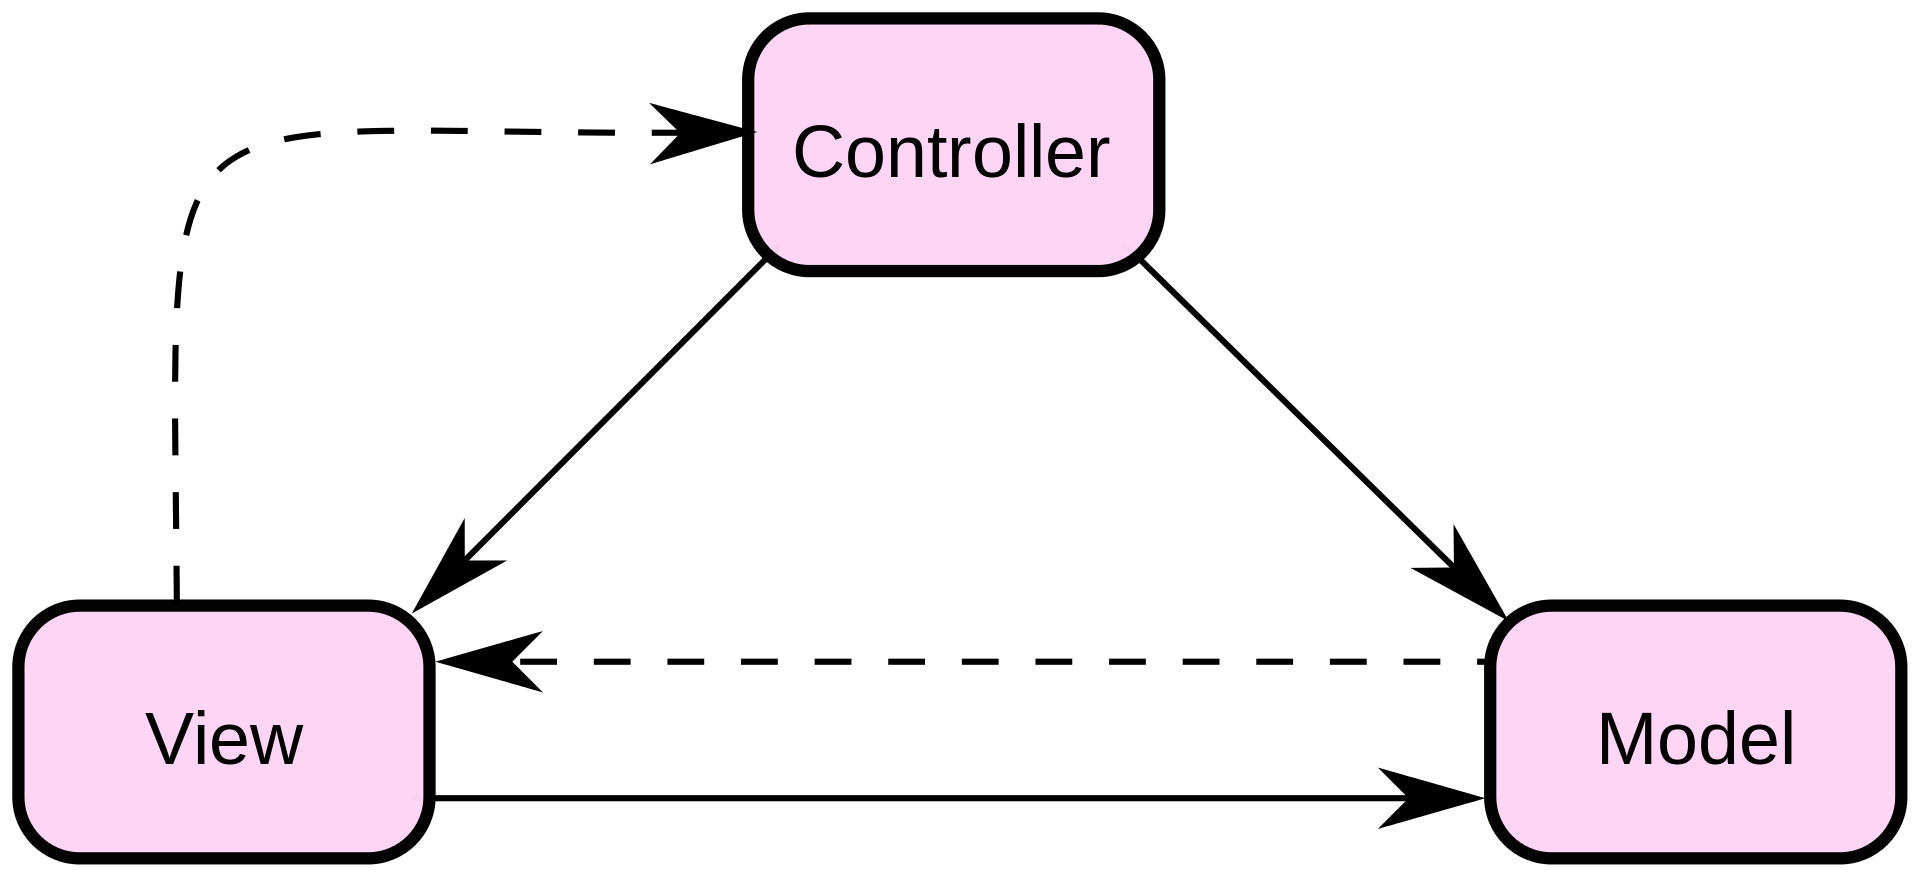
\includegraphics[scale=0.15]{imagens/mvc.png}}
	\legend{Fonte: \url{https://pt.wikipedia.org/wiki/MVC}}
	\label{fig:mvc}
\end{figure}

\subsection{O que faz cada camada?}

As camadas do \textbf{Padrão de Design MVC} possuem cada uma sua responsabilidade. Tais responsabilidades são listas abaixo:

\begin{itemize}[leftmargin=1.7cm]
	\setlength\itemsep{0em}
	\item \textbf{Controladores - Controllers}: Um Controller representa as classes que conectam o modelo e a visão e é usado para comunicação entre as classes no \textbf{modelo} e na \textbf{visão}.
	\item \textbf{Visualizações - Views}: Uma View é uma coleção de classes que representam os elementos na interface do usuário (todas as coisas que o usuário pode ver e responder na tela, como botões, caixas de exibição e assim por diante)
	\item \textbf{Modelos - Models}: Um modelo representa a estrutura lógica subjacente de dados em um aplicativo de software e a classe de alto nível associada a ele. Este modelo de objeto não contém nenhuma informação sobre a interface do usuário.
\end{itemize}

Assim, para podermos usar a estrutura MVC em nossos projetos, devemos usar uma ferramenta que possibilite as conexões listas acima. Para tanto, vamos usar um em específico, o \textbf{ExpressJS}.

\section{Express Web Framework}

Alguns problemas surgem quando vamos desenvolver. No exercício anterior, para criarmos uma página simples, conseguimos resolver facilmente. Contudo, caso queiramos uma organização ou apenas criar uma página a tarefa é bem mais complicada. Assim, para resolver esses problemas, que não são apenas nossos, mas comuns durante o desenvolvimento profissional, foram criadas ferramentas cujo objetivo é facilitar a codificação e reduzir a repetição de código. Uma dessas é o \textbf{Framework ExpressJS}. 

\begin{citacao}
	Assim um \textbf{Framework} tem como principal objetivo resolver problemas recorrentes com uma abordagem genérica, permitindo ao desenvolvedor focar seus esforços na resolução do problema em si, e não ficar reescrevendo software \cite{mozzila}. 
\end{citacao}

Express é um popular framework web estruturado, escrito em JavaScript que roda sobre o ambiente NodeJS em tempo de execução. Este módulo explica alguns dos principais benefícios deste framework, como configurar o seu ambiente de desenvolvimento e como executar tarefas comuns de desenvolvimento e implantação da web.

\subsection{Instalando o ExpressJS}

Para realizar a instalação do ExpressJS vamos seguir o Guia presente em \url{https://expressjs.com/pt-br/starter/installing.html}. Assumindo que já tenha instalado o Node.js, crie um diretório para conter o seu aplicativo, e torne-o seu diretório ativo iniciando um projeto usando o \textbf{Yarn} como feito em \ref{usando_yarn}.

Para instalar o express usando o seguinte comando:

\begin{minted}[frame=single,framesep=10pt,breaklines,linenos,tabsize=2,autogobble]{bash}
	yarn add express
\end{minted}

\subsection{Exemplo Hello World}
Para nosso primeiro exemplo vamos continuar usando o Guia citado anteriormente \url{https://expressjs.com/pt-br/starter/hello-world.html}. No diretório criado crie um arquivo chamado \textbf{index.js} e inclua o seguinte código:

\begin{minted}[frame=single,framesep=10pt,breaklines,linenos,tabsize=2,autogobble]{javascript}
	const express = require('express')
	const app = express()
	const port = 3000
	
	app.get('/', (req, res) => {
		res.send('<h1>Hello World!</h1>')
	})
	
	app.listen(port, () => {
		console.log(`Servidor escutando na porta ${port}`)
	})
\end{minted}

Também modifique o \textbf{package.json} adicionado o \textbf{Script} para iniciar o projeto usando o \textbf{nodemon}. Não se esqueça de instalar o \textbf{nodemon} em desenvolvimento.

\section{Usando Embedded Javascript Templating (ejs)}

Se você estiver escrevendo um aplicativo \textit{Server Side} em Node.js e quiser enviar HTML de volta para os clientes com conteúdos dinâmicos, você deve encontrar uma maneira de misturar ou interpolar os dados. O EJS (Embedded JavaScript Templating) é um dos mecanismos de modelo mais populares para JavaScript. Como o nome sugere, ele nos permite incorporar código JavaScript em uma linguagem de modelo que é então usada para gerar HTML.

Um mecanismo de modelo é um software projetado para combinar modelos de dados para produzir, no nosso caso, código HTML real.

\begin{figure}[H]
	\centering
	\caption{Mecanismos de modelo}
	\frame{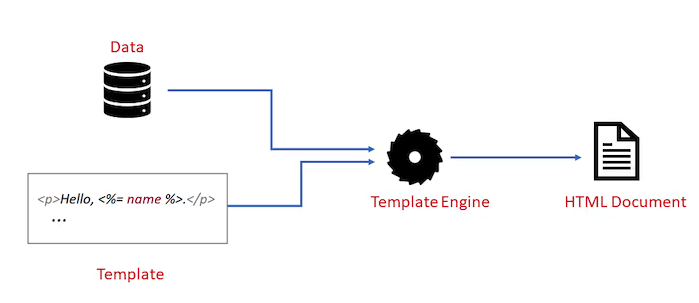
\includegraphics[scale=0.6]{imagens/modelo-ejs.png}}
\end{figure}

Os mecanismos de modelo lidam com a tarefa de interpolar dados em código HTML enquanto fornecem alguns recursos (como parciais em EJS) que seriam difíceis de replicar concatenando strings.

\subsection{Instalando e configurando o EJS}

Para instalar e configurar o EJS em nosso projeto, devemos, primeiramente, instalar a biblioteca que fornecerá o suporte em nossa aplicação e criar um diretório, na raiz do projeto, com o nome de \textbf{views}.

\begin{minted}[frame=single,framesep=10pt,breaklines,linenos,tabsize=2,autogobble]{javascript}
	yarn add ejs
	npm install ejs
\end{minted}

Agora, com a dependência já instalada, vamos configurar a nossa aplicação para usar o EJS. Isso tudo será feito dentro do nosso arquivo \textbf{index.js.}

\begin{minted}[frame=single,framesep=10pt,breaklines,linenos,tabsize=2,autogobble]{javascript}
	const express = require('express')
	const path = require('path');
	const app = express();
	const port = 3000
	
	app.use(express.static('public'));
	app.set('view engine', 'ejs');
	
	app.get('/', (req, res) => {
		res.render('index');
	})
	
	app.listen(port, () => {
		console.log(`Servidor executando na porta ${port}`)
	})
\end{minted}

E, no diretório \textbf{views}, criaremos um arquivo que será o utilizado para a exibição com o nome de \textbf{index.ejs}.

\subsection{Passando dados para serem renderizados}

Lembre-se de que nosso objetivo é combinar dados com modelos. Podemos fazer isso passando um segundo argumento para res.render. Este segundo argumento deve ser um objeto, que estará acessível no arquivo de modelo EJS.

Para tanto, adicione o seguinte código no arquivo \textbf{index.js}

\begin{minted}[frame=single,framesep=10pt,breaklines,linenos,tabsize=2,autogobble]{javascript}
	const express = require('express')
	const path = require('path');
	const app = express();
	const port = 3000
	
	app.use(express.static('public'));
	app.set('view engine', 'ejs');
	
	const usuario = {
		nome: 'Luiz',
		sobrenome: 'Picolo',
	}
	
	app.get('/', (req, res) => {
		res.render('index', {
			usuario
		})
	})
	
	app.listen(port, () => {
		console.log(`Servidor executando na porta ${port}`)
	})
\end{minted}

E no arquivo \textbf{index.ejs} inclua o objeto da seguinte forma:

\begin{minted}[frame=single,framesep=10pt,breaklines,linenos,tabsize=2,autogobble]{javascript}
	<h1>Olá, eu sou o <%= usuario.nome  %></h1>
\end{minted}

\subsection{Exercício de fixação}

1) Crie um rota de artigos. Depois, crie uma lista de postagens (como se fosse um blog) e liste-as ao acessar a rota artigos. Lembre-se de criar o arquivo EJS como feito anteriormente. 

\section{Requisições de objetos: req.params e req.query}

Até o momento, todos os dados que trafegaram em nossos estudos foram apenas do Servidor para o Cliente. Agora, a ideia é transmitir dados do Cliente para o Servidor. Para isso, vamos usar as três expressões descritas acima, req.body, req.query e req.params, que fazem parte do \textbf{Objeto de solicitação no Express.js} e são usados, pelo cliente, para enviar dados para o servidor. A princípio, vamos trabalhar com dados vindos das URLs.

\subsection{req.params}

O \textbf{req.params} tem com objetivo capturar propriedades anexadas ao URL, ou seja, parâmetros de rota nomeados. Você prefixa o nome do parâmetro com dois pontos (:) ao escrever suas rotas. Por exemplo, vamos capturar o parâmetro da URL abaixo:

\textbf{http://localhost:3000/artigos/123}

Assim, nossa rota artigos deve ser modificada da seguinte forma:

\begin{minted}[frame=single,framesep=10pt,breaklines,linenos,tabsize=2,autogobble]{javascript}
app.get('/artigos/:numero', (req, res) => {
	console.log(req.params.numero)
})	
\end{minted}

Caso houvesse mais parâmetros, poderíamos fazer da seguinte forma:

\textbf{http://localhost:3000/artigos/123/titulo}

\begin{minted}[frame=single,framesep=10pt,breaklines,linenos,tabsize=2,autogobble]{javascript}
	app.get('/artigos/:numero/:titulo', (req, res) => {
		console.log(req.params.numero)
		console.log(req.params.titulo)
	})	
\end{minted}

\subsection{req.query}

Já o req.query é usado principalmente para pesquisa, classificação, filtragem, paginação, etc. Digamos, que desejássemos obter a mesma URL anterior mas usando o query, ou, que tivessemos 10, 15 parâmetros. A escrita da rota ficaria comprometida pela dificuldade de entendimento. Assim, podemos rescrever tanto a \textbf{URL} como a \textbf{rota} ela usando o \textbf{req.query}. 

\textbf{http://localhost:3000/artigos?numero=123\&titulo=titulo-do-artigo}

\textbf{Observe com atenção}

Perceba que, após a rota é usando um ponto de interrogação, e, para separar os demais parâmetros, usando o \& também conhecido com E comercial.

\begin{minted}[frame=single,framesep=10pt,breaklines,linenos,tabsize=2,autogobble]{javascript}
	app.get('/artigos', (req, res) => {
		console.log(req.query.numero)
		console.log(req.query.titulo)
	})	
\end{minted}

\subsection{Exercício de Fixação}

1) A partir das URLs abaixo, crie suas respectivas rotas e, usando os conceitos aprendidos na aula anterior, apresente os parâmetros em um arquivos EJS.

\begin{itemize}[leftmargin=1.7cm]
	\setlength\itemsep{0em}
	\item http://localhost:3000/girafa?altura=15\&nome=juju
	\item http://localhost:3000/girafa/15/juju
	\item http://localhost:3000/noticias?id=123
	\item http://localhost:3000/noticias/123
\end{itemize}

2) Vamos usar as rotas para calcular o Teorema de Pitágoras. Use a seguinte URL para criar a rota e os parâmetros:

http://localhost:3000/pitagoras?a=4\&b=6\&c=3

\begin{figure}[H]
	\centering
	\frame{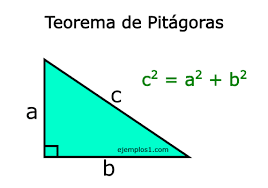
\includegraphics[scale=0.6]{imagens/pitagoras.png}}
\end{figure}
\chapter{Introdução}

\section{O que é JavaScript}

O JavaScript foi criado na década de 90 por \textbf{Brendan Eich} a serviço da 
Netscape (uma empresa de serviços de computadores nos EUA a qual era mais 
conhecida pelo seu navegador, o Netscape). Essa década foi um período de 
``revolução'', pois os navegadores ainda eram estáticos sendo o mais popular 
dessa época o Mosaic, da NCSA.

\begin{figure}[H]
  \centering
  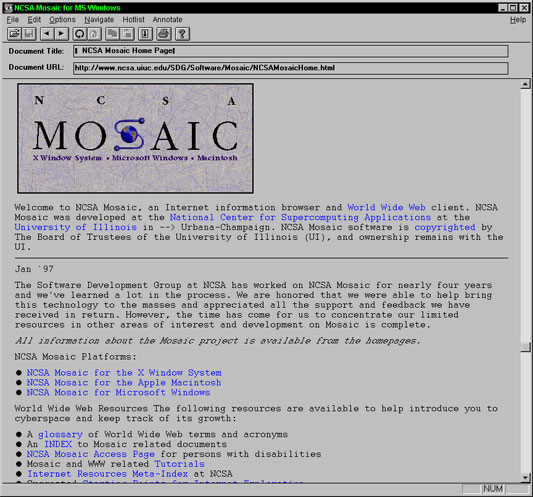
\includegraphics[scale=0.6]{imagens/mosaic_beta.jpg}
  \caption{NCSA Mosaic versão beta}
  \legend{Fonte: \cite{historyComputer}}
  \label{fig:historyComputer}
\end{figure}

O JavaScript foi introduzido em 1995 como uma forma de adicionar programas às 
páginas web do navegador Netscape. A linguagem, desde então, foi adotada por 
todos os outros grandes navegadores web que possuem interfaces gráficas. Ele 
tornou as aplicações modernas possíveis, fazendo com que você não tenha que 
recarregar a página inteira quando for necessário realizar interações diretas 
com a aplicação. Além disso, ele é usado em páginas web mais tradicionais, 
fornecendo diferentes maneiras de criar interatividade e inteligência \cite
{haverbeke2014eloquent}.

\section{ECMAScript ou JavaScript?}

Depois que o JavaScript foi adotado fora do Netscape, um documento padrão foi 
escrito para descrever a maneira na qual a linguagem deveria funcionar, 
garantindo que as diferentes partes dos softwares que afirmavam suportar 
JavaScript estavam, de fato, falando sobre a mesma linguagem. Esse documento é 
chamado de padrão ECMAScript, nomeado pela organização internacional Ecma, que 
foi responsável pela padronização. Na prática, os termos ECMAScript e 
JavaScript podem ser usados como sinônimos, pois são dois nomes para a mesma 
linguagem.

Na prática, existem diversos softwares que suportam JavaScript e possuem seu 
comportamente semelhante. Os navegadores, ou browsers, são exemplos destes 
tipos de software os quais implementam a linguagem por meio das especificações 
regidas pelo ECMAScript. Outro mais atual é o NodeJS ou simplesmente Node 
(https://nodejs.org/) que busca executar o JavaScript diretamente no servidor 
(Node será aprofundado em capítulos posteriores).

Para constatar este fato, execute o seguinte código no console em diferentes 
navegadores: 

\begin{lstlisting}
alert('Bem vindo(a) ao JavaScript')
\end{lstlisting}

O código acima possui o mesmo comportamento? Sim, o comportamento é o mesmo em 
todos os navegadores. Contudo, a forma gráfica com que é apresentado faz parte 
da implementação feita. Portanto, o desenvolvedor pode utilizar o JavaScript 
nos navegadores sem muito problema, pois eles seguem não ideias da equipe que o 
criou mas uma especificação que dita as regras de como determinadas funções 
devem se comportar.

\section{Versões do JavaScript ou edições ECMAScript}

Como foi visto, o ECMAScript é apenas a especificação. Contudo, ao estudar a 
linguagem é muito comum escutar a abreviação de ECMAScript, ou seja, ES. Assim, 
sempre que se ler ES seguido de um número, esse está fazendo referência a uma 
edição do ECMAScript. Atualmente, existem oito edições do ECMAScript publicadas,
sendo que, a partir de 2015, as edições começaram a receber o ano e não mais o 
número da edição.

\begin{enumerate}
  \item ECMAScript 1 (1997)	
  \item ECMAScript 2 (1998)	
  \item ECMAScript 3 (1999)	
  \item ECMAScript 4	Nunca foi lançada.
  \item ECMAScript 5 (2009)
    \begin{enumerate}[label*=\arabic*.]
    \item ECMAScript 5.1 (2011)
    \end{enumerate}
  \item ECMAScript 2015
  \item ECMAScript 2016
  \item ECMAScript 2017
  \item ECMAScript 2018
\end{enumerate}

\section{Conclusão}
Portanto, JavaScript se tornou a linguagem de programação mais popular no 
desenvolvimento Web sendo suportada por todos os navegadores e responsável por 
praticamente qualquer tipo de dinamismos em páginas web. Ao se usar todo o 
poder que ela tem para oferecer, pode-se chegar a resultados impressionantes. 
Alguns excelentes exemplos disso são aplicações Web complexas como Gmail, 
Google Maps e Google Docs. 

\setcounter{chapter}{1}
\chapter{O que é User Experience (UX)}

\begin{flushright}
	\textit{
		UX é pesquisar sobre os usuários de modo que você possa dar para eles \\ o que eles precisam para conseguirem algo que querem.
	} \\
	
	\textbf{autor desconhecido}
\end{flushright}


No Capítulo \ref{cap:cap1}, nós realizamos a introdução sobre alguns conceitos norteadores da Interação Humano-Computador (IHC). No meio de todos os conceitos apresentados, algo se destaca em meio ao material apresentado, que é \textbf{usuário}. Sem dúvida, podemos afirmar que, o usuário, mediante sua interação com os sistemas computacionais, é a base para que uma área de estudo como IHC pudesse ser construída.

Já neste capítulo, iremos tratar não somente da interação do usuário por meios das interfaces, mas também da qualidade da sua experiência ao usar elas.

\section{Experiência do usuário}

Segundo \citeonline{teixeira2014introduccao}, a experiência do usuário existe desde que o mundo é mundo. Desde que as pessoas começaram a ``usar' objetos para realizar alguma tarefa podemos dizer que existe um contexto de experiências. Experiências são subjetivas. Cada pessoa tem uma experiência diferente ao usar um caixa eletrônico, um aplicativo, uma rede social, entre outros. Essa experiência, segundo \citeonline{teixeira2014introduccao} é influenciada por dois tipos de fatores: \textbf{humanos} e \textbf{externos} 

Como \textbf{fatores humanos} podemos citar as habilidade em usar caixas eletrônicos, por exemplo. Sua visão, sua habilidade motora, sua capacidade de ler e entender o que está escrito na tela, seu humor naquele momento, entre outros fatos. Já como \textbf{fatores externos}, podemos citar o horário do dia, o ambiente onde o caixa eletrônico está instalado, o fato de ter uma fila de pessoas atrás do utilizador, e assim por diante.

Assim, podemos dizer que o tema experiência do usuário é um tema bastante subjetivo. É difícil de maneira objetiva e direta dizer como desenhar uma experiência do usuário, mas é possível aprendermos como desenhar um produto, serviço ou ambiente que proporcione uma experiência satisfatória para alguém que os use, identificando todos os aspectos da interação do usuário com esse produto (ou serviço ou ambiente).

Portanto, a experiência do usuário está ligado a forma com que a pessoa se sente ao usar um produto. Ou mais formalmente, de acordo com a definição dada pela ISO 9241-210, são as respostas e percepções de uma pessoa resultantes do uso de um produto, sistema ou serviço.

UX designers trabalham para construir produtos que sejam fáceis de usar
(a tal \textbf{usabilidade}), reduzindo a fricção e permitindo que os usuários completem a tarefa desejada em menos tempo, com menos ruído e obstáculos.

\begin{figure}[H]
	\centering
	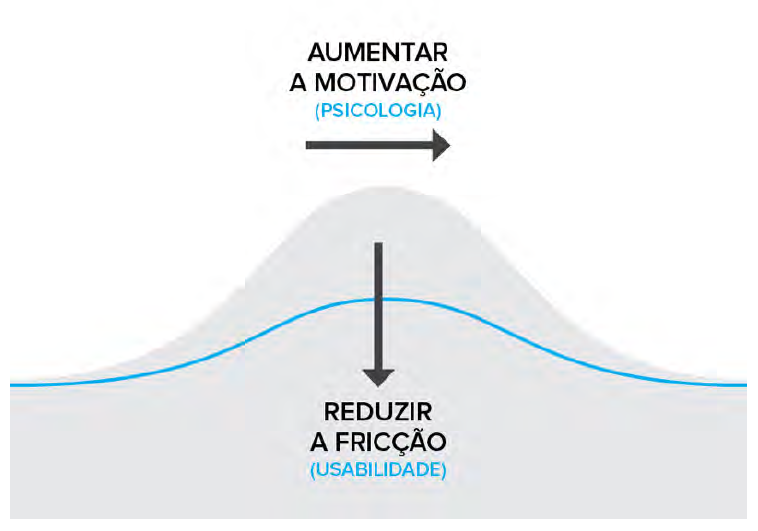
\includegraphics[scale=0.4]{imagens/aumento-friqcao.png}
	\caption{Stephen Anderson. Livro Seductive Interaction Design}
	%\legend{Fonte: \cite{IrlaRebelo}}
	%\label{fig:interface-interacao}
\end{figure}

\subsection{Usabilidade e a experiência do usuário}

Segundo a norma sobre requisitos de ergonomia, ISO 9241-11 (1998), define usabilidade como sendo: \textit{O grau em que um produto é usado por usuários específicos para atingir objetivos
específicos com \textbf{eficácia}, \textbf{eficiência} e \textbf{satisfação} em um contexto de uso
específico.}

\begin{itemize}
	\item \textbf{eficácia}: está relacionada com a capacidade de os usuários interagirem com o sistema para alcançar seus objetivos corretamente, conforme o esperado;
	
	\item \textbf{eficiência}:  está relacionada com os recursos necessários para os usuários
	interagirem com o sistema e alcançarem seus objetivos. Normalmente, os recursos
	necessários são tempo, mão de obra e materiais envolvidos; 
	
	\item \textbf{satisfação}: A norma também destaca
	a importância de considerarmos o grau de contentamento dos usuários com a experiência
	de usar o sistema interativo no contexto de uso para o qual foi projetado.
\end{itemize} 

De forma mais simplificada, segundo \cite{teixeira2014introduccao}: usablidade é garantir que as interfaces sejam fáceis de usar. Que o usuário consiga realizar uma tarefa sem transtorno ou demora em um número
razoável de passos, como também, toda informações sejam fáceis de entender e de fácil acesso. 

\section{Métodos e entregáveis em UX}

Quando falamos em métodos e entregáveis, os profissionais da área costumam ter uma série itens que gostam de utilizar: wireframes, sitemaps, user journeys, análise comparativa de funcionalidades, entre vários outros. Contudo, neste capítulo, vamos abordar apenas três os quais acreditamos ser os mais utilizados que são: \textbf{Brainstorming, Personas, Entrevistas com Stakeholders, Wireframes e Sitemaps}.

\subsection{Brainstorming}

O processo coletivo de geração de ideias, sem restrições. Uma sessão de \textit{brainstorming} busca
levantar de forma bastante livre um conjunto grande e abrangente de opiniões dos
participantes em torno de um tema. Os resultados dessa atividade podem alimentar
diretamente a especificação funcional e documentação de design \cite{barbosa2010IHC}.

\subsection{Personas}

Para \citeonline{teixeira2014introduccao}, personas é  um retrato do público-alvo que destaca dados demográficos, comportamentos,
necessidades e motivações por meio da criação de um personagem ficcional
baseado em \textit{insights} extraídos de pesquisa. Personas fazem com que os designers e desenvolvedores criem empatia com os consumidores durante o processo de design.

\begin{figure}[H]
	\centering
	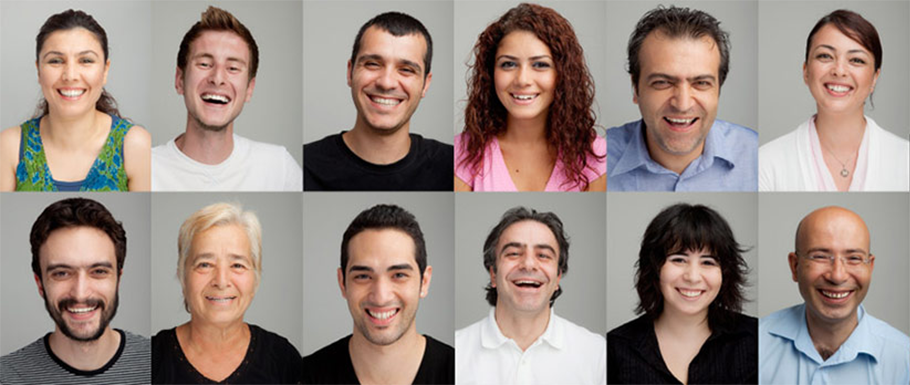
\includegraphics[scale=0.4]{imagens/personas-marketing.png}
	\caption{Exemplo de personas}
	\legend{Fonte: http://www.altgrupo.com.br/blog/marketing-digital-por-que-investir-no-uso-de-personas/}
	%\label{fig:interface-interacao}
\end{figure}

Para definir uma persona, \citeonline{courage2005understanding} enumera os seguintes elementos característicos:

\begin{itemize}
	\item \textbf{identidade}: dê a uma persona nome e sobrenome. Forneça uma idade e outros dados demográficos que seriam representativos do perfil do usuário. Inclua também uma foto, para tornar a persona ainda mais realista e memorável;
	\item \textbf{status}: defina se esta persona é primária, secundária, outro \textit{stakeholder} ou representa um antiusuário do seu sistema. Um antiusuário é alguém que não vai utilizar o produto e, portanto, não deve influenciar as decisões de projeto;
	\item \textbf{objetivos}: quais são os objetivos desta persona? Não se limite a objetivos relacionados ao seu produto específico;
	\item \textbf{habilidades}: qual é a especialidade da sua persona? Isso inclui educação, treinamento e competências específicas. Novamente, não se limite a detalhes relacionados ao seu produto específico;
	\item \textbf{tarefas}: em linhas gerais, quais as tarefas básicas ou críticas que a persona realiza? Qual é a frequência, importância e duração dessas tarefas?;
	\item \textbf{relacionamentos}: entender com quem a persona se relaciona é importante, pois ajuda a identificar outros \textit{stakeholders};
	\item \textbf{requisitos}: de que a persona precisa? Inclua citações que ajudam a dar mais vida a essas necessidades;
	\item \textbf{expectativas}: como a persona acredita que o produto funciona? Como ela organiza as informações no seu domínio ou trabalho?
\end{itemize}

Embora personas sejam fictícias, elas são definidas com rigor e detalhes para representar usuários ``típicos''. Elas são derivadas de um processo de investigação que levanta as características dos usuários e descreve seus perfis \cite{barbosa2010IHC}.

\subsubsection{Diferença entre persona e público-alvo}

Para \citeonline{riandutra2018} um erro bastante esta no fato da não diferenciação de personas de público-alvo. O público-alvo é algo mais genérico, abrangente, enquanto a persona é mais humanizada e personalizada.

Por exemplo, um público-alvo poderia ser: homens e mulheres, entre 30 e 40 anos, casados, com ensino médio completo, com renda mensal de até 15.000 reais. Têm até dois filhos e pretendem comprar uma casa de veraneio para a família.

Agora, um exemplo de persona: Patrícia, 31 anos, não tem filhos, é solteira, formada em design e pós-graduada em animação 3D. Busca ascensão profissional na empresa em que trabalha há cerca de dois anos. Gostaria de morar sozinha e procura formas de poupar dinheiro para as despesas de um novo apartamento.





\chapter{Definição sobre JavaScript Object Notation (JSON)}\label{cap:cap3}

\begin{flushright}
	\textit{
		Um ladrão rouba um tesouro, mas não furta a inteligência. \\
		Uma crise destrói um herança, mas não uma profissão. \\ Não importa se você não tem dinheiro, você é uma pessoa rica, \\ pois possui o maior de todos os capitais: a sua inteligência. \\ Invista nela. \textbf{Estude}!.
	} \\
	
	\textbf{Augusto Cury}
\end{flushright}

JSON (JavaScript Object Notation) é um formato de intercâmbio de dados leve. É fácil para que seres humanos possam ler e escrever. É fácil para que as máquinas possam analisar e gerar. É baseado em um subconjunto do \textbf{Padrão de Linguagem de Programação JavaScript ECMA-262 3ª Edição} - Dezembro de 1999. JSON é um formato de texto completamente independente da linguagem, mas usa convenções que são familiares aos programadores da família C de linguagens, incluindo C, C ++, Java, JavaScript, Perl, Python e muitos outros. Essas propriedades tornam o JSON uma linguagem de intercâmbio de dados ideal\footnote{Para mais detalhes acesse: https://www.json.org/json-pt.html}.

Json também é um formato baseado em texto padrão para representar dados estruturados com base na sintaxe do objeto JavaScript. É comumente usado para transmitir dados em aplicativos da Web (por exemplo, enviar alguns dados do servidor para o cliente, para que possam ser exibidos em uma página da Web ou vice-versa). Você se deparará com isso com bastante frequência, portanto, neste artigo, oferecemos tudo o que você precisa para trabalhar com o JSON usando JavaScript, incluindo a análise do JSON para que você possa acessar os dados dentro dele e criar o JSON\footnote{Para mais detalhes acesse: \url{https://developer.mozilla.org/pt-BR/docs/Learn/JavaScript/Objects/JSON}}.

\section{Estrutura JSON}

Um JSON é uma string cujo formato se parece muito com o formato literal do objeto JavaScript. Você pode incluir os mesmos tipos de dados básicos dentro do JSON, como em um objeto JavaScript padrão — strings, números, matrizes, booleanos e outros literais de objeto. Isso permite que você construa uma hierarquia de dados. 

\begin{lstlisting}
let Retangulo = {
	"largura": 100,
	"altura": 100
}

let Retangulos = [
	{"largura": 100, "altura": 100},
	{"largura": 200, "altura": 200},
]
\end{lstlisting}

Assim, para realizar o acesso aos dados de um objeto Json, usamos a mesma notação \textbf{dot} / \textbf{bracket} usada em objetos literais.

\begin{lstlisting}
let Retangulo = {
	"largura": 100,
	"altura": 100
}

let Retangulos = [
	{"largura": 100, "altura": 100},
	{"largura": 200, "altura": 200},
]

console.log(Retangulo.largura)
console.log(Retangulo['largura'])

console.log(Retangulos[0].largura)
console.log(Retangulo[0]['largura'])
\end{lstlisting}

Contudo, o Json recebido venha em formato de String, ele deverá ser convertido para um objeto JavaScript. Assim, usando a função \textbf{JSON.parse()} podemos converter a string em um objeto, da seguinte forma:

\begin{lstlisting}
let retangulo = Json.parse('{"largura": 100, "altura": 100}')
console.log(Retangulo.largura)
\end{lstlisting}

\section{Exercícios de Fixação}

\begin{enumerate}
	\item No exercício 2.4 criamos uma classe \textbf{Noticia} que continha alguns atributos (titulo, dataDaPublicacao, resumo e texto) e uma outra classe \textbf{NoticiaDestaque} que continha, além dos atributos citados, um atributo imagem. Assim, baseando-se nos atributos listados, crie um arquivo \textbf{json} com nome \textbf{noticias.json} e atribua a ele uma lista de notícias no formato estudado. O arquivo deve conter no mínimo 5 notícias.
\end{enumerate}

\section{Obtendo JSON de um servidor web (Requisição Ajax)}

Para obter o JSON, vamos usar uma API chamada \textbf{XMLHttpRequest} (geralmente chamada de XHR). Esse é um objeto JavaScript muito útil que nos permite fazer solicitações de rede para recuperar recursos de um servidor via JavaScript (por exemplo, imagens, texto, JSON e até trechos de código HTML), o que significa que podemos atualizar pequenas seções de conteúdo sem ter que recarregar todo página. Isso levou a páginas da Web mais responsivas e parece empolgante, mas está além do escopo deste artigo ensinar isso com muito mais detalhes\footnote{Para mais detalhes acesse: \url{https://developer.mozilla.org/pt-BR/docs/Learn/JavaScript/Objects/JSON}}.

Para começar, vamos armazenar a URL do JSON que queremos recuperar em uma variável. Adicione o seguinte na parte inferior do seu código JavaScript:

\begin{lstlisting}
	let requestURL = 'https://raw.githubusercontent.com/luizpicolo/json-for-testing
/main/dragonball.json';
\end{lstlisting}

Para criar uma solicitação, precisamos criar uma nova instância de objeto de solicitação a partir do construtor XMLHttpRequest usando a palavra-chave new. Adicione o seguinte abaixo sua última linha:

\begin{lstlisting}
	let request = new XMLHttpRequest();
\end{lstlisting}

Agora precisamos abrir uma nova solicitação usando o método open() . Adicione a seguinte linha:

\begin{lstlisting}
	request.open('GET', requestURL);
\end{lstlisting}

Isso leva pelo menos dois parâmetros — existem outros parâmetros opcionais disponíveis. Nós só precisamos dos dois obrigatórios para este exemplo simples:

\begin{itemize}
	\item O método HTTP a ser usado ao fazer a solicitação de rede. Neste caso, GET é bom, pois estamos apenas recuperando alguns dados simples.
	\item O URL para fazer a solicitação — esta é a URL do arquivo JSON que armazenamos anteriormente.
\end{itemize}

Em seguida, adicione as duas linhas a seguir — aqui estamos definindo o  responseType como JSON, para que o XHR saiba que o servidor retornará o JSON e que isso deve ser convertido nos bastidores em um objeto JavaScript. Em seguida, enviamos a solicitação com o método send():

\begin{lstlisting}
	request.responseType = 'json';
	request.send();
\end{lstlisting}

A última parte desta seção envolve aguardar a resposta retornar do servidor e, em seguida, lidar com ela. Adicione o seguinte código abaixo do seu código anterior:

\begin{lstlisting}
	request.onload = function() {
		let personagens = request.response;
		
		const elemento = document.getElementById('list');
		let p1 = personagens.characters[0].name;
		elemento.insertAdjacentHTML('afterbegin', p1);
	}
\end{lstlisting}

\section{Exercícios de Fixação}

\begin{itemize}
	\item A partir do arquivo \textbf{noticias.json} criado no exercício anterior, e utilizando também as classes \textbf{Noticia} e \textbf{NoticiaDestaque} implementadas, leia e apresente no navegador as notícias contidas no arquivo \textbf{noticias.json}. Para tanto, você deve utilizar implementar a leitura do arquivo e, a partir dos dados, criar objetos e apresentar os mesmos no navegador. Abaixo segue o modelo base para o desenvolvimento do trabalho
\end{itemize}
\chapter{Versionamento de Código}\label{cap:cap3}

\begin{flushright}
	\textit{
		Um ladrão rouba um tesouro, mas não furta a inteligência. \\
		Uma crise destrói um herança, mas não uma profissão. \\ Não importa se você não tem dinheiro, você é uma pessoa rica, \\ pois possui o maior de todos os capitais: a sua inteligência. \\ Invista nela. \textbf{Estude}!.
	} \\
	
	\textbf{Augusto Cury}
\end{flushright}

De forma simples, podemos dizer que o controle de versão é um sistema que registra as mudanças feitas em um arquivo ou um conjunto de arquivos ao longo do tempo de forma que você possa recuperar versões específicas para praticamente qualquer tipo de arquivo em um computador. 

Assim, esse capítulo, tem como objetivo proporcionar a você leitor(a) os pontos os quais julgamos mais importantes para compreender e praticar o controle de versão. Esse tipo de técnica é amplamente utilizado em ambientes de trabalho, nos quais, várias pessoas tem que trabalhar em um mesmo projeto. Assim, caso um erro aconteça, ou características nova surjam, os membros da equipe podem corrigir o problema de forma simples e rápida.  

\section{Projeto de banco de dados}


\chapter{Autenticação e autorização com JWT}


%\input{cap6}

% ----------------------------------------------------------
% Finaliza a parte no bookmark do PDF
% para que se inicie o bookmark na raiz
% e adiciona espaço de parte no Sumário
% ----------------------------------------------------------
\phantompart

% ---
% Conclusão
% ---
%\chapter{Conclusão}
% ---

% ----------------------------------------------------------
% ELEMENTOS PÓS-TEXTUAIS
% ----------------------------------------------------------
\postextual
% ----------------------------------------------------------

% ----------------------------------------------------------
% Referências bibliográficas
% ----------------------------------------------------------
\bibliography{referencias.bib}

% ----------------------------------------------------------
% Glossário
% ----------------------------------------------------------
%
% Consulte o manual da classe abntex2 para orientações sobre o glossário.
%
%\glossary

%\include{apendices}

%\include{anexos}

%---------------------------------------------------------------------
% INDICE REMISSIVO
%---------------------------------------------------------------------
\phantompart
\printindex
%---------------------------------------------------------------------

\end{document}
